Ben Trout

2014-14-14

Building

\begin{tabular}{|p{5cm}|p{5cm}|}
\hline
Building Launcher&
At the beginning of the week we had an intake and that’s about it. As the next step, building the launcher, got under way we split into two groups. David and Nick started to wire the whole robot while me, Filip, and Matt started to build the launcher. The idea is simple. We have a bar attached with a gear ratio to a motor. The bar has another cardboard piece to it that hits the balls. Our gear ratio is a 3:1 allowing the cardboard to hit the balls with more force. We put the bar higher up allowing us to have a longer piece of cardboard. We also put the launcher at the front of our robot taking of our original intake. 
\\
\hline
\end{tabular}

\section*{Building Launcher}
Building the new launcher was easy. It was basically a replica of the intake just had a swapped gear ratio to make it go faster. It didn’t take us long though to realize that having an intake and then a launcher that were identical was inefficient. We didn’t need an intake if all we had to do is drive around and hit the balls with our launcher. We originally had the launcher behind the intake and as the intake took in the balls the launcher would spin around and hit them up a makeshift ramp we made. We had many problems with this: from the two cardboard pieces hitting each other to the balls getting stuck under the cardboard as it swung around. We took of both the intake and launcher at this point. We put the launcher at the very front of the robot putting it two bars higher than before allowing us to have a larger piece of cardboard. By moving it to the front we have all that space in the back available now for the ramp. By moving the axel up two bars we won’t have to worry about the balls getting stuck under the cardboard as it can swing out farther and scoop them in. Next week we’ll focus on building the ramp we’ll be flinging the balls up. 

\begin{center}
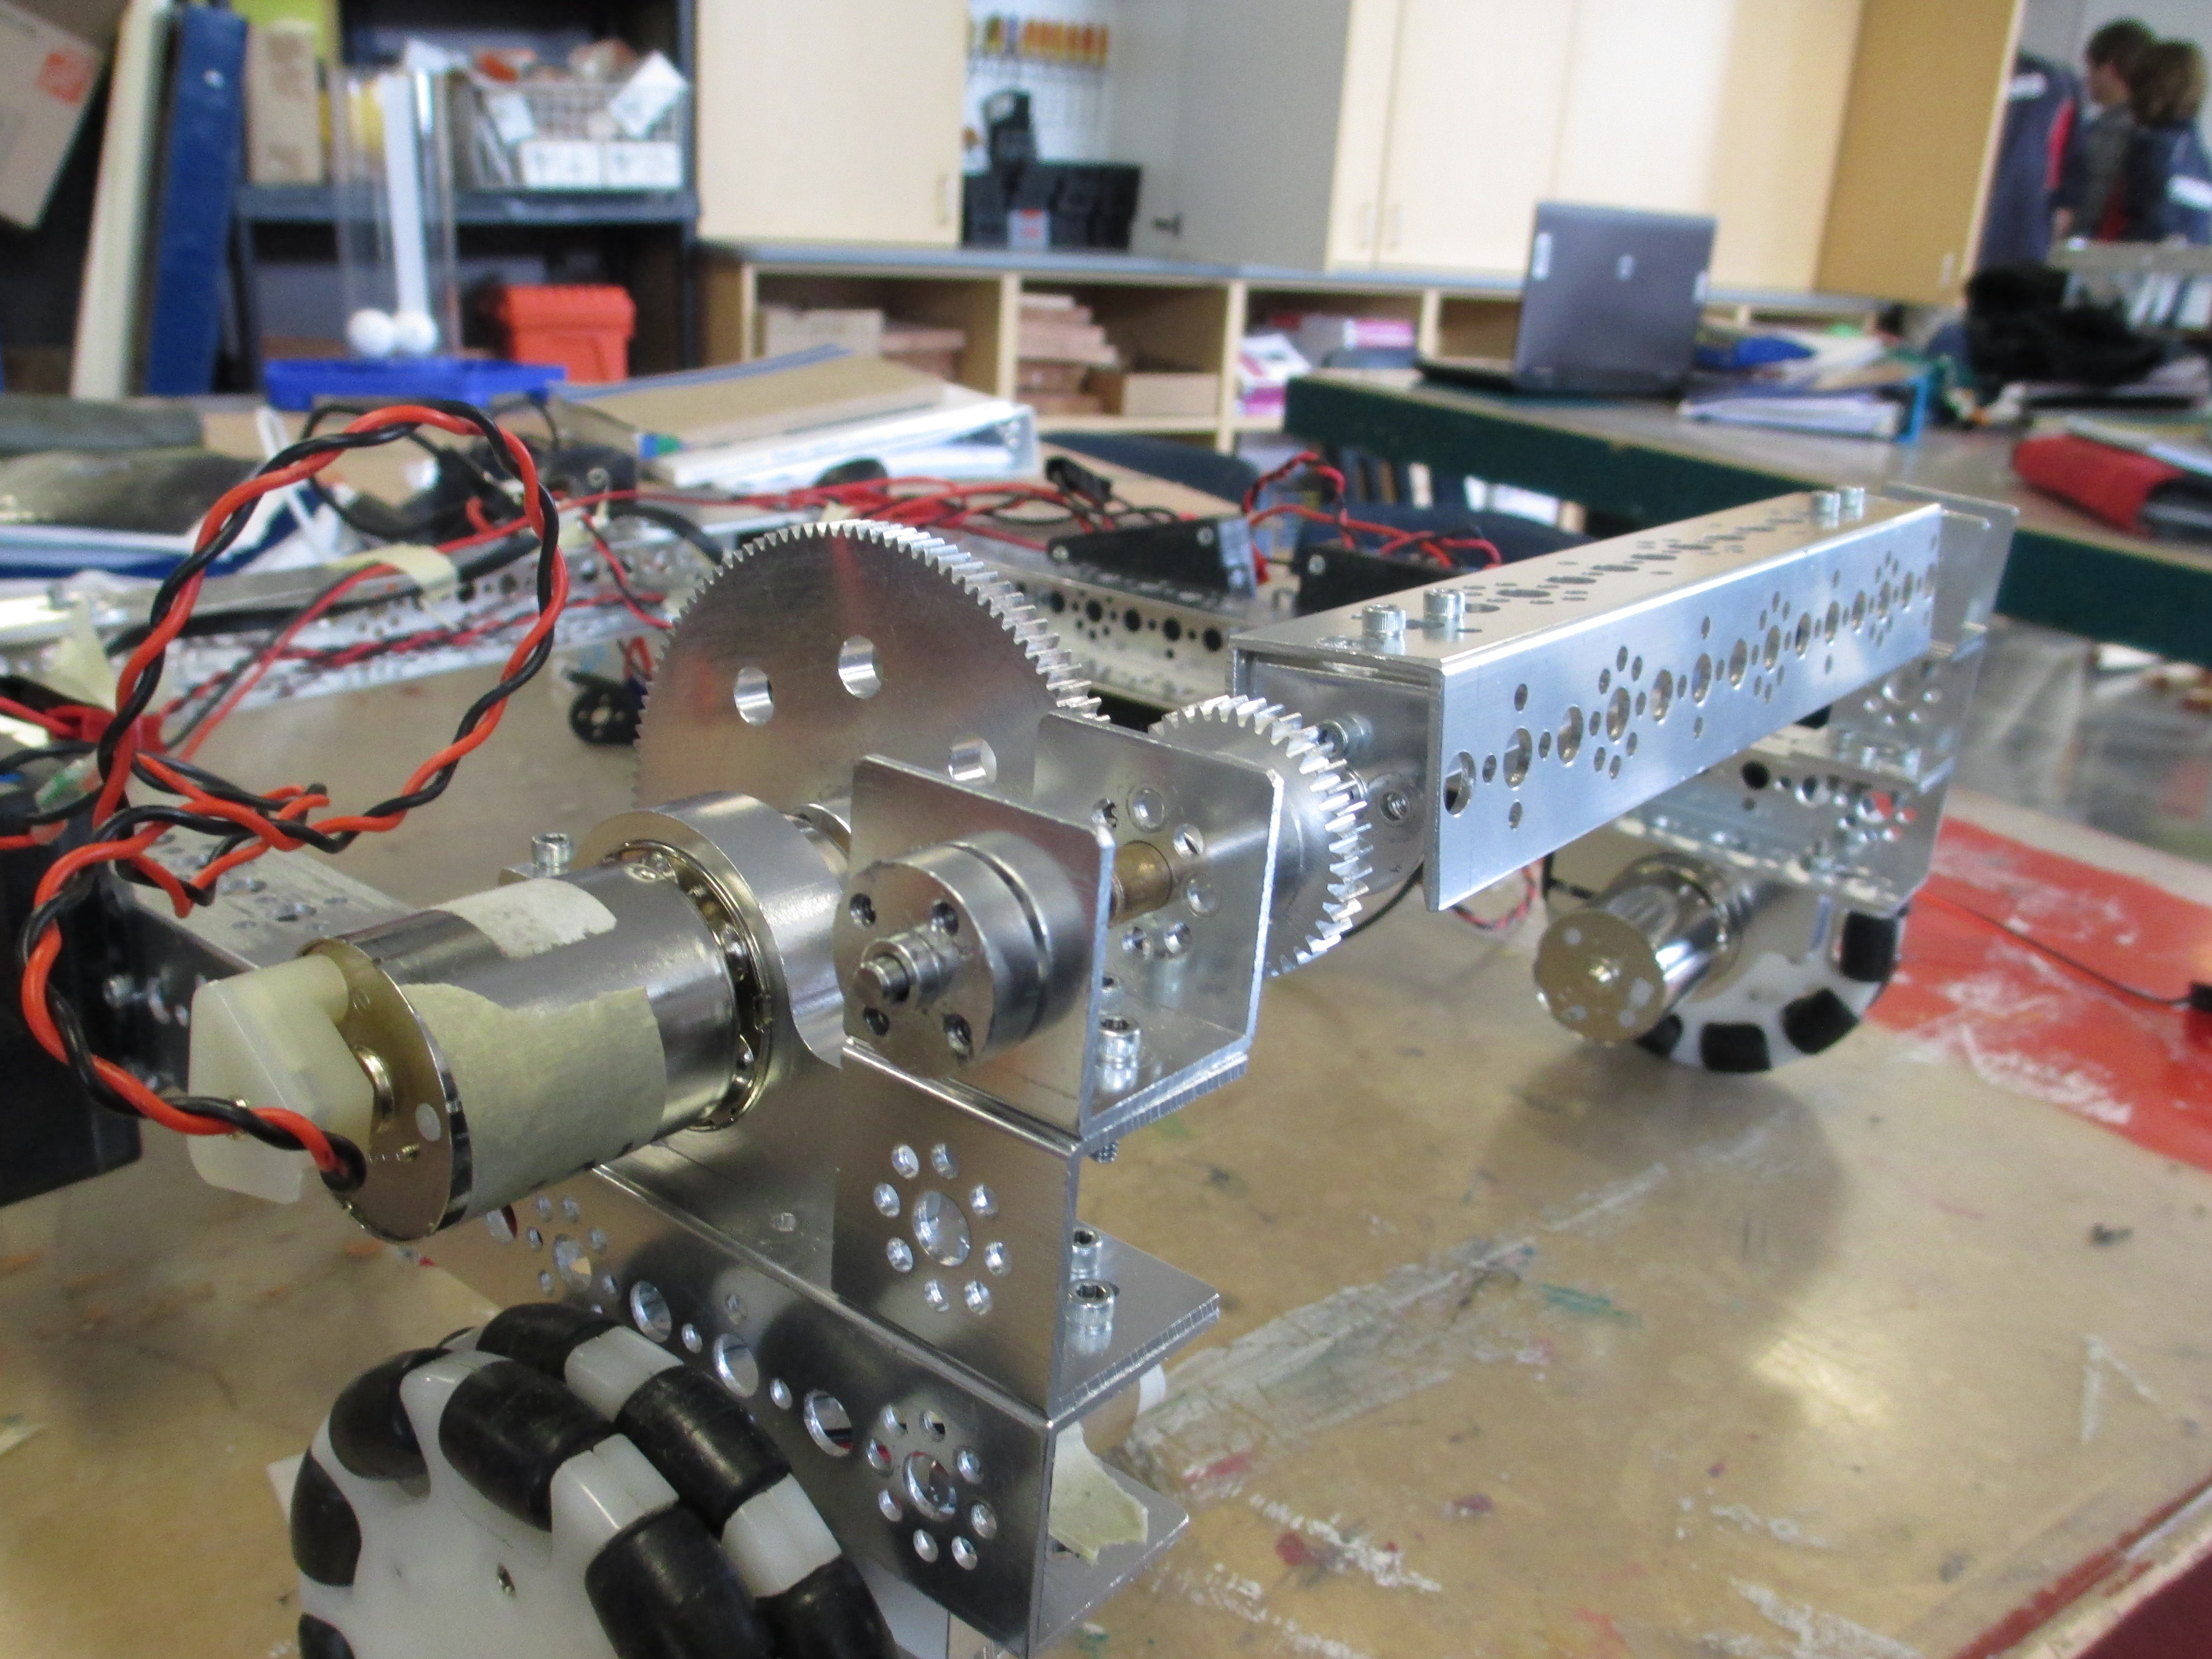
\includegraphics[width=10cm]{./Entries/Images/LauncherInFront.jpg}
\end{center}
